\documentclass{report} 
\title{Bondy \& Murty}
\date{Started 13th October 2025}
\author{Malcolm}
\usepackage{amsmath} %import math
\usepackage{mathtools} %more math
\usepackage{amssymb} %for QED symbol
\usepackage{amsthm} %
\usepackage{mathrsfs} %
\usepackage{bm}%bold math
\usepackage{graphicx} %import imaging

\graphicspath{{./images/}} %set imaging path
\newtheorem*{theorem}{Theorem}
\theoremstyle{definition}
\newtheorem*{definition}{Definition}


\begin{document}
\maketitle

\tableofcontents

\newpage
\chapter{Graphs}
\section{Definitions and examples}
A \textit{graph} is an ordered pair $(V(G),E(G))$ consisting of a set $V(G)$ of \textit{vertices} and a set $E(G)$, disjoint from $V(G)$, of \textit{edges}, together with an 
\textit{incidence function} $\psi_G$ that associates with each edge of $G$ an unordered pair of (not necessarily distinct) vertices of $G$.\\
\vspace{1mm}\\
If $e$ is an edge and $u$ and $v$ are vertices such that $\psi_G(e)=\{u,v\}$ then $e$ is said to \textit{join} $u$ and $v$, and the vertices $u$ and $v$ are called the \textit{ends} of $e$.\\
\vspace{1mm}\\
We denote the numbers of vertices and edges in $G$ by $v(G)$ and $e(G)$; these two basic parameters are called the \textit{order} and \textit{size} of $G$ respectively.\\
\vspace{1mm}\\
\textbf{Example 1}\\
These examples serve to clarify the definition. For notational simplicity, we write $uv$ for the unordered pair $\{u,v\}$.
\begin{equation*}
G=(V(G),E(G))
\end{equation*}
where
\begin{align*}
&V(G)=\{u,v,w,x,y\}\\
&E(G)=\{a,b,c,d,e,f,g,h\}
\end{align*}
and $\psi_G$ is defined by
\begin{align*}
&\psi_G(a)=uv\quad\psi_G(b)=uu\quad\psi_G(c)=vw\quad\psi_G(d)=wx\\
&\psi_G(e)=vx\quad\psi_G(f)=wx\quad\psi_G(g)=ux\quad\psi_G(h)=xy
\end{align*}
(next page)\newpage
\noindent\textbf{Example 2}
\begin{equation*}
H=(V(H),E(H))
\end{equation*}
where
\begin{align*}
&V(H)=\{v_0,v_1,v_2,v_3,v_4,v_5\}\\
&E(H)=\{e_1,e_2,e_3,e_4,e_5,e_6,e_7,e_8,e_9,e_{10}\}
\end{align*}
and $\psi_H$ is defined by
\begin{align*}
\psi_H(e_1)=v_1v_2\quad&\psi_H(e_2)=v_2v_3\quad\psi_H(e_3)=v_3v_4\quad\psi_H(e_4)=v_4v_5\\
\psi_H(e_5)=v_5v_1\quad&\psi_H(e_6)=v_0v_1\quad\psi_H(e_7)=v_0v_2\quad\psi_H(e_8)=v_0v_3\\
&\psi_H(e_9)=v_0v_4\quad\psi_H(e_{10})=v_0v_5
\end{align*}
\textbf{Drawings and more definitions}\\
Graphs are so named because they can be represented graphically. Each vertex is indicated by a point and each edge by a line joining the points representing its ends. Here are the graphs of the two
given examples:
\begin{center}
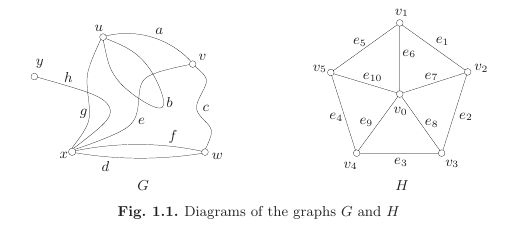
\includegraphics[width=10cm]{1}\\
\end{center}
There is no single correct way to draw a graph; the relative positions of the points representing vertices and the shapes of lines representing edges usually have no significance. A diagram of
a graph merely depicts the incidence relation between its vertices and edges.\\
\vspace{1mm}\\
The ends of an edge are said to be \textit{incident} with the edge and vice versa. Two vertices incident with a common edge are \textit{adjacent}, as are two edges which are incident with a 
common vertex, and two distinct adjacent vertices are \textit{neighbours}. The set of neighbours of a vertex $v$ in a graph $G$ is denoted by $N_G(v)$.\\
\vspace{1mm}\\
An edge with identical ends is called a \textit{loop}, and an edge with distinct ends a \textit{link}. Two or more links with the same pair of ends are said to be \textit{parallel edges}.
For instance in the graph $G$ of the first example, the edge $b$ is a loop, and all other edges are links; the edges $d$ and $f$ are parallel edges.\\
(next page)\newpage
\noindent\textbf{Cont.}\\
We use $G$ to denote a graph. But when there is no scope for ambiguity, we omit the letter $G$ from graph-theoretic symbols and write, for instance, $V$ and $E$ for $V(G)$ and $E(G)$. 
We also denote the numbers of vertices and edges of $G$ by $n$ and $m$ respectively.\\
\vspace{1mm}\\
A graph is \textit{finite}





















\end{document}
